
\chapter{Multivariate Analysis in Metabolomics}

\begin{quote}
{\it Essentially, all models are wrong, but some are useful.}
\\\\
 -- George E. P. Box
\end{quote}

\section{Introduction}

\begin{doublespace}
The applications of chemometrics are as broad as the field of chemistry itself,
but one particularly challenging subdiscipline of bioanalytical chemistry --
known as ``metabolomics'' -- has recently renewed interest in the use of
chemometrics \cite{worley:cmb2013}. Indeed, the chemical complexity of
systems studied by metabolomics {\it necessitates} the use of chemometric
techniques: if metabolomics were a nail, chemometrics would surely be a hammer.
\\\\
Metabolomics is defined \cite{lindon:cmr2000} as ``the quantitative
measurement of the multiparametric metabolic response of living systems to
pathophysiological stimuli or genetic modification.'' Such a definition implies
that metabolomics studies offer the finest-grained detail available in the
nascent field of systems biology: a molecular-level convolution of all upstream
genomic, transcriptomic and proteomic responses of an organism to a given
stimulus or change
\cite{kell:opin2004,trethewey:opin2001,weckwerth:arpb2003}. Metabolites
are the end product of all cellular processes, and their in vivo
concentrations are a direct result of enzymatic activity. While a change in the
expression level of a protein or its coding gene may not necessarily correlate
directly with the activity of that protein, alterations in metabolite
concentrations {\it are} the consequence of altered activity
\cite{terkuile:febs2001}. Thus, metabolites are more proximal to a
phenotype or disease state than either genetic or proteomic information. The
richness of phenotypic information offered by metabolomics has been leveraged
to identify disease biomarkers
\cite{gebregiworgis:cchts2012,vinayavekhin:acscb2010}, to aid in
the drug discovery process \cite{powers:mrc2009,wilcoxen:eodd2010}, and to
study plants \cite{hall:pcell2002}, bacteria
\cite{zhang:jiomic2013,tang:cgen2011}, nutrition
\cite{mcniven:jnb2011}, and the environment
\cite{bundy:metab2009}, among numerous other applications
\cite{baker:nmeth2011}.
\\\\
The rich information promised by metabolomics does not come without a price,
and metabolomics experiments are plagued with difficulty. The number of
small-molecule metabolites in a biofluid, cell lysate, tissue or organ differs
wildly depending on the organism studied, ranging from several hundered to
hundreds of thousands \cite{dunn:trac2005}. While databases of commonly
encountered metabolites have been compiled
\cite{wishart:nar2007,cui:nbiot2008,kind:anchem2009}, they are by no
means complete. Therefore, it is common to encounter unknown signals during
data analysis, complicating the interpretation of metabolic changes between
experimental groups. Metabolite identification is further complicated by a
lack of NMR or mass spectral reference information for known metabolites.
Finally, the diversity of chemical and physical properties of metabolites
makes true simultaneous quantitation of all metabolites present in a system
unattainable with current instrumental capabilities
\cite{lindon:cmr2000,dunn:trac2005,dettmer:msr2007}. As an illustration,
due to the limited molecular mass distribution of the metabolome, comprehensive
metabolomic analyses by mass spectrometry generally require the prefixing of
one or more chromatographic separations prior to analyte ionization
\cite{kell:opin2004,viswanadhan:acsccc2011}.
\\\\
The extraction of information from data in metabolomics experiments is further
complicated by the inherent variability present within each sample. Every
single cell, tissue, organ or organism is fundamentally unique
\cite{rubakhin:nmeth2011}, despite any features (disease state, drug
treatment, {\it etc.}) it may have in common with others of its kind. Thus,
the differentiation between two experimental groups in a metabolomics
experiment requires the identification of relatively few defining or
discriminating chemical features against a large, complex background of
metabolites \cite{wishart:nar2007}. Ideally, these few chemical features
may be identified as a unique set of metabolites that are directly related to
the defining biochemical states of each experimental group. Unfortunately, all
biological systems are easily perturbed by experimental or environmental
factors, including age, gender, diet, cell growth phase, nutrient availability,
pH and temperature \cite{tyagi:ijpsrr2010,zhang:jiomic2013}. Variations in
sample handling procedures, including cell lysis, metabolic quenching,
metabolite extraction and sample storage can also introduce further variability
into the measured data. Finally, variations in signal position, intensity and
shape may manifest from instrumental instabilities on a per-sample basis.
Each of these numerous sources of sample variability increases the magnitude of
$\mathbf{E}$ in any chemometric model that may be applied to the data
(cf. \hyperlink{section.1.1}{Section 1.1}), which decreases the statistical
validity of $f(\mathbf{D})$. Therefore, the design of experiments and analysis
of data in metabolomics requires robust methodologies in order to expose
underlying chemical trends from highly complex systems in the form of
statistically valid mathematical models. This chapter describes the theory
and best practices of chemometric analyses of data produced by metabolomics
experiments, with a focus on 1D \hnmr{} and 2D \hcnmr{} NMR datasets.
\end{doublespace}

\begin{figure}[ht!]
\begin{center}
  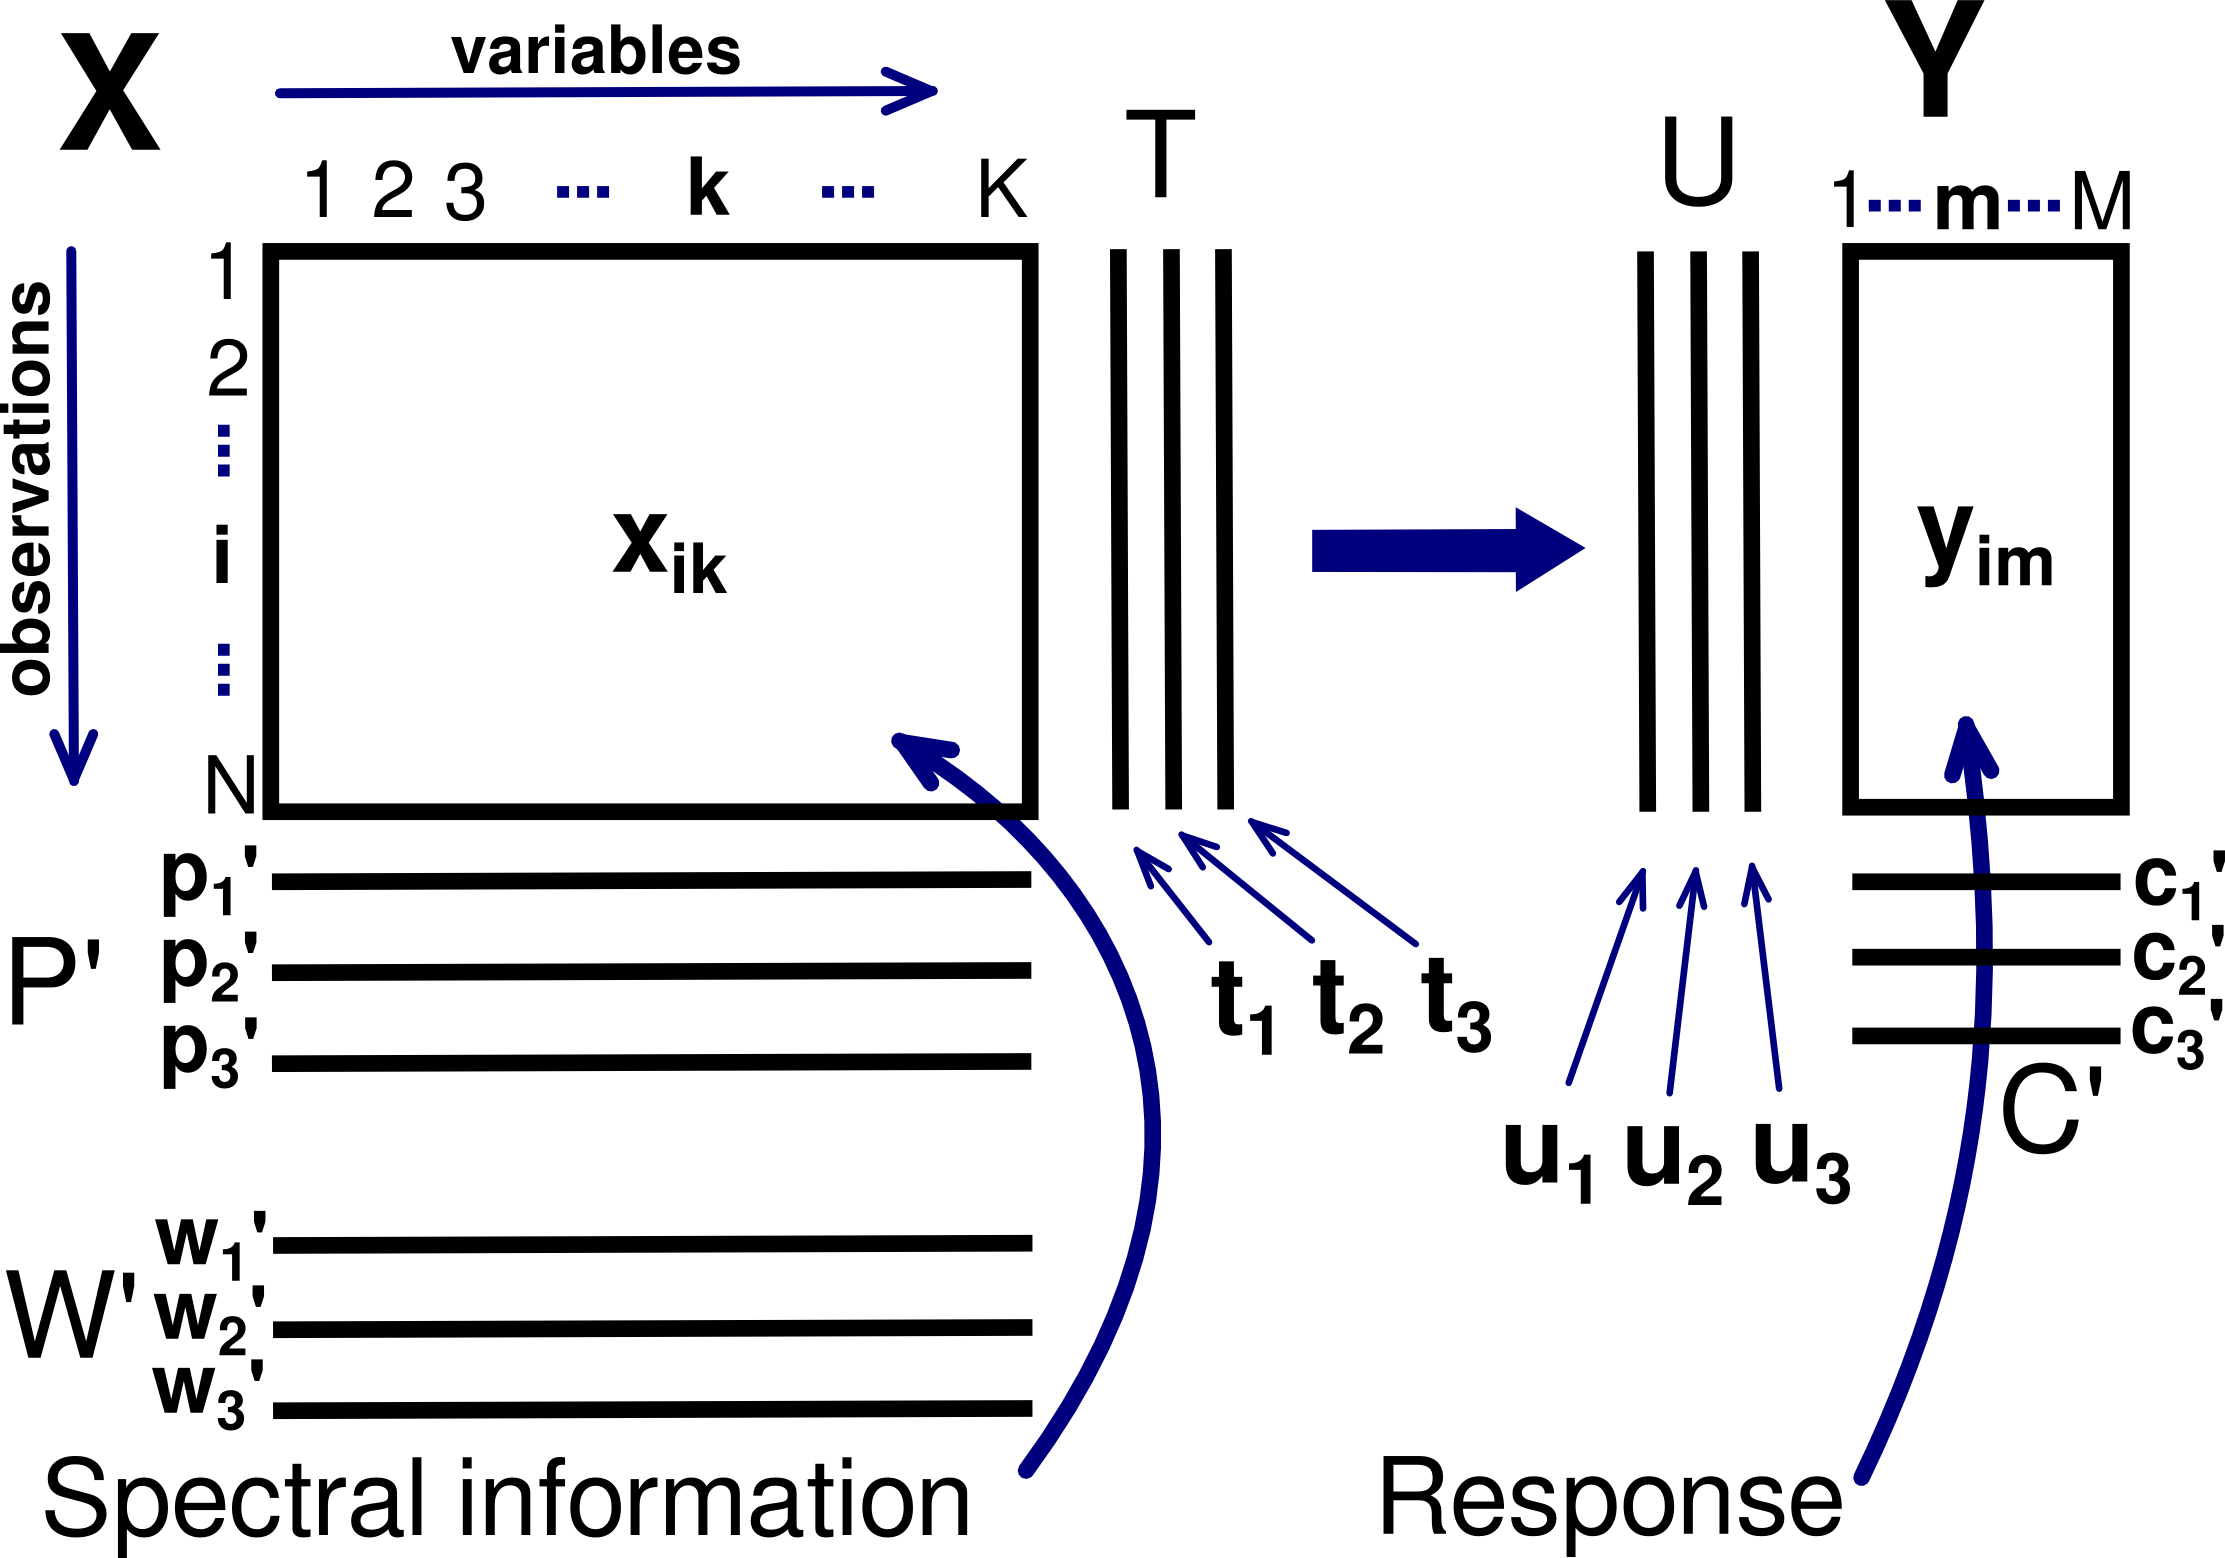
\includegraphics[width=4in]{figs/mva/01.png}
\end{center}
\caption
      [Canonical Example of a Bilinear Modeling Problem.]{
  {\bf Canonical Example of a Bilinear Modeling Problem.}
  \\
  Illustration of a data matrix $\mathbf{X}$ and a response matrix
  $\mathbf{Y}$, as they are typically used in partial least squares
  modeling problems. In metabolomics applications, the data matrix will
  contain a set of $N$ spectra, each having $K$ variables. For supervised
  modeling problems, each observation in the data matrix is paired with a
  corresponding row in the response matrix that holds either continuously
  varying outputs or binary class memberships. The data are then decomposed
  into a small number of score vectors ($\mathbf{t}$) and loading vectors
  ($\mathbf{p}$), with corresponding weight vectors ($\mathbf{w}$) used
  to transform the observations in $\mathbf{X}$ into scores-space. The
  responses in $\mathbf{Y}$ are similarly decomposed into scores
  ($\mathbf{u}$) and loadings ($\mathbf{c}$). Tick marks denote
  transposition.
}
\end{figure}

\section{Multivariate Datasets}

\begin{doublespace}
In the majority of cases, multivariate datasets used in metabolomics take the
form of second-order tensors in $\mathbb{R}^{N \times K}$. More simply, these
datasets are real matrices having $N$ rows and $K$ columns. By convention,
the data are arranged as $N$ observation row vectors of length $K$, where $K$
is referred to as the dimensionality of the dataset (Figure 3.1). Typical
examples of 1D datasets include sets of \hnmr{} or \cnmr{} NMR spectra
\cite{beckonert:nprot2007,koh:colon2009}, direct-injection mass spectra
(DI-MS, \cite{castrillo:phch2003,southam:anchem2007,zhou:asms2010}), infrared
(IR) and Raman spectra \cite{ellis:analyst2006,cherney:anchem2007}, or
capillary electrophoretograms (CE, \cite{ramautar:trac2006}). This remarkable
diversity of instrumental platforms used in metabolomics is traceable to the
ability of bilinear factorizations such as principal component analysis
(PCA, \cite{jolliffe2002}) and partial least squares (PLS, \cite{wold1993}) to
directly accept these second-order tensors for modeling (vide infra).
\\\\
The dimensionality of a multivariate dataset may be increased by adding another
``mode'', resulting in a third-order (or higher) tensor
($\mathbf{X} \in \mathbb{R}^{N \times K_1 \times K_2}$, Figure 3.2). In such
cases, the total dimensionality of the dataset is now the product of the
dimensionalities along each mode of the data tensor (e.g. $K_1 \times K_2$).
Third-order tensors are the natural data structures for sets of two-dimensional
observations, including \hhnmr{}, \hcnmr{} and \hnnmr{} NMR spectra, hyphenated
chromatography-mass spectra (LC-MS, GC-MS), hyphenated electrophoresis-mass
spectra (CE-MS), and hyphenated ion-mobility mass spectra (IM-MS). While
third-order data tensors may hold substantially more chemical information than
their second-order counterparts, they are not directly compatible with bilinear
factorization methods, and they require specialized processing,
treatment and modeling algorithms \cite{lu:ieee2009,lu:pr2011}. As an example,
tensors may be vectorized into matrices \cite{hedenstrom:cils2008} that are
suited for PCA and PLS, but at the cost of lost structural information. Methods
such as uncorrelated multilinear PCA (UMPCA, \cite{lu:ieee2009}), on the other
hand, provide a means of directly decomposing tensors into low-dimensional
spaces while maintaining structural information.
\end{doublespace}

\begin{SCfigure}
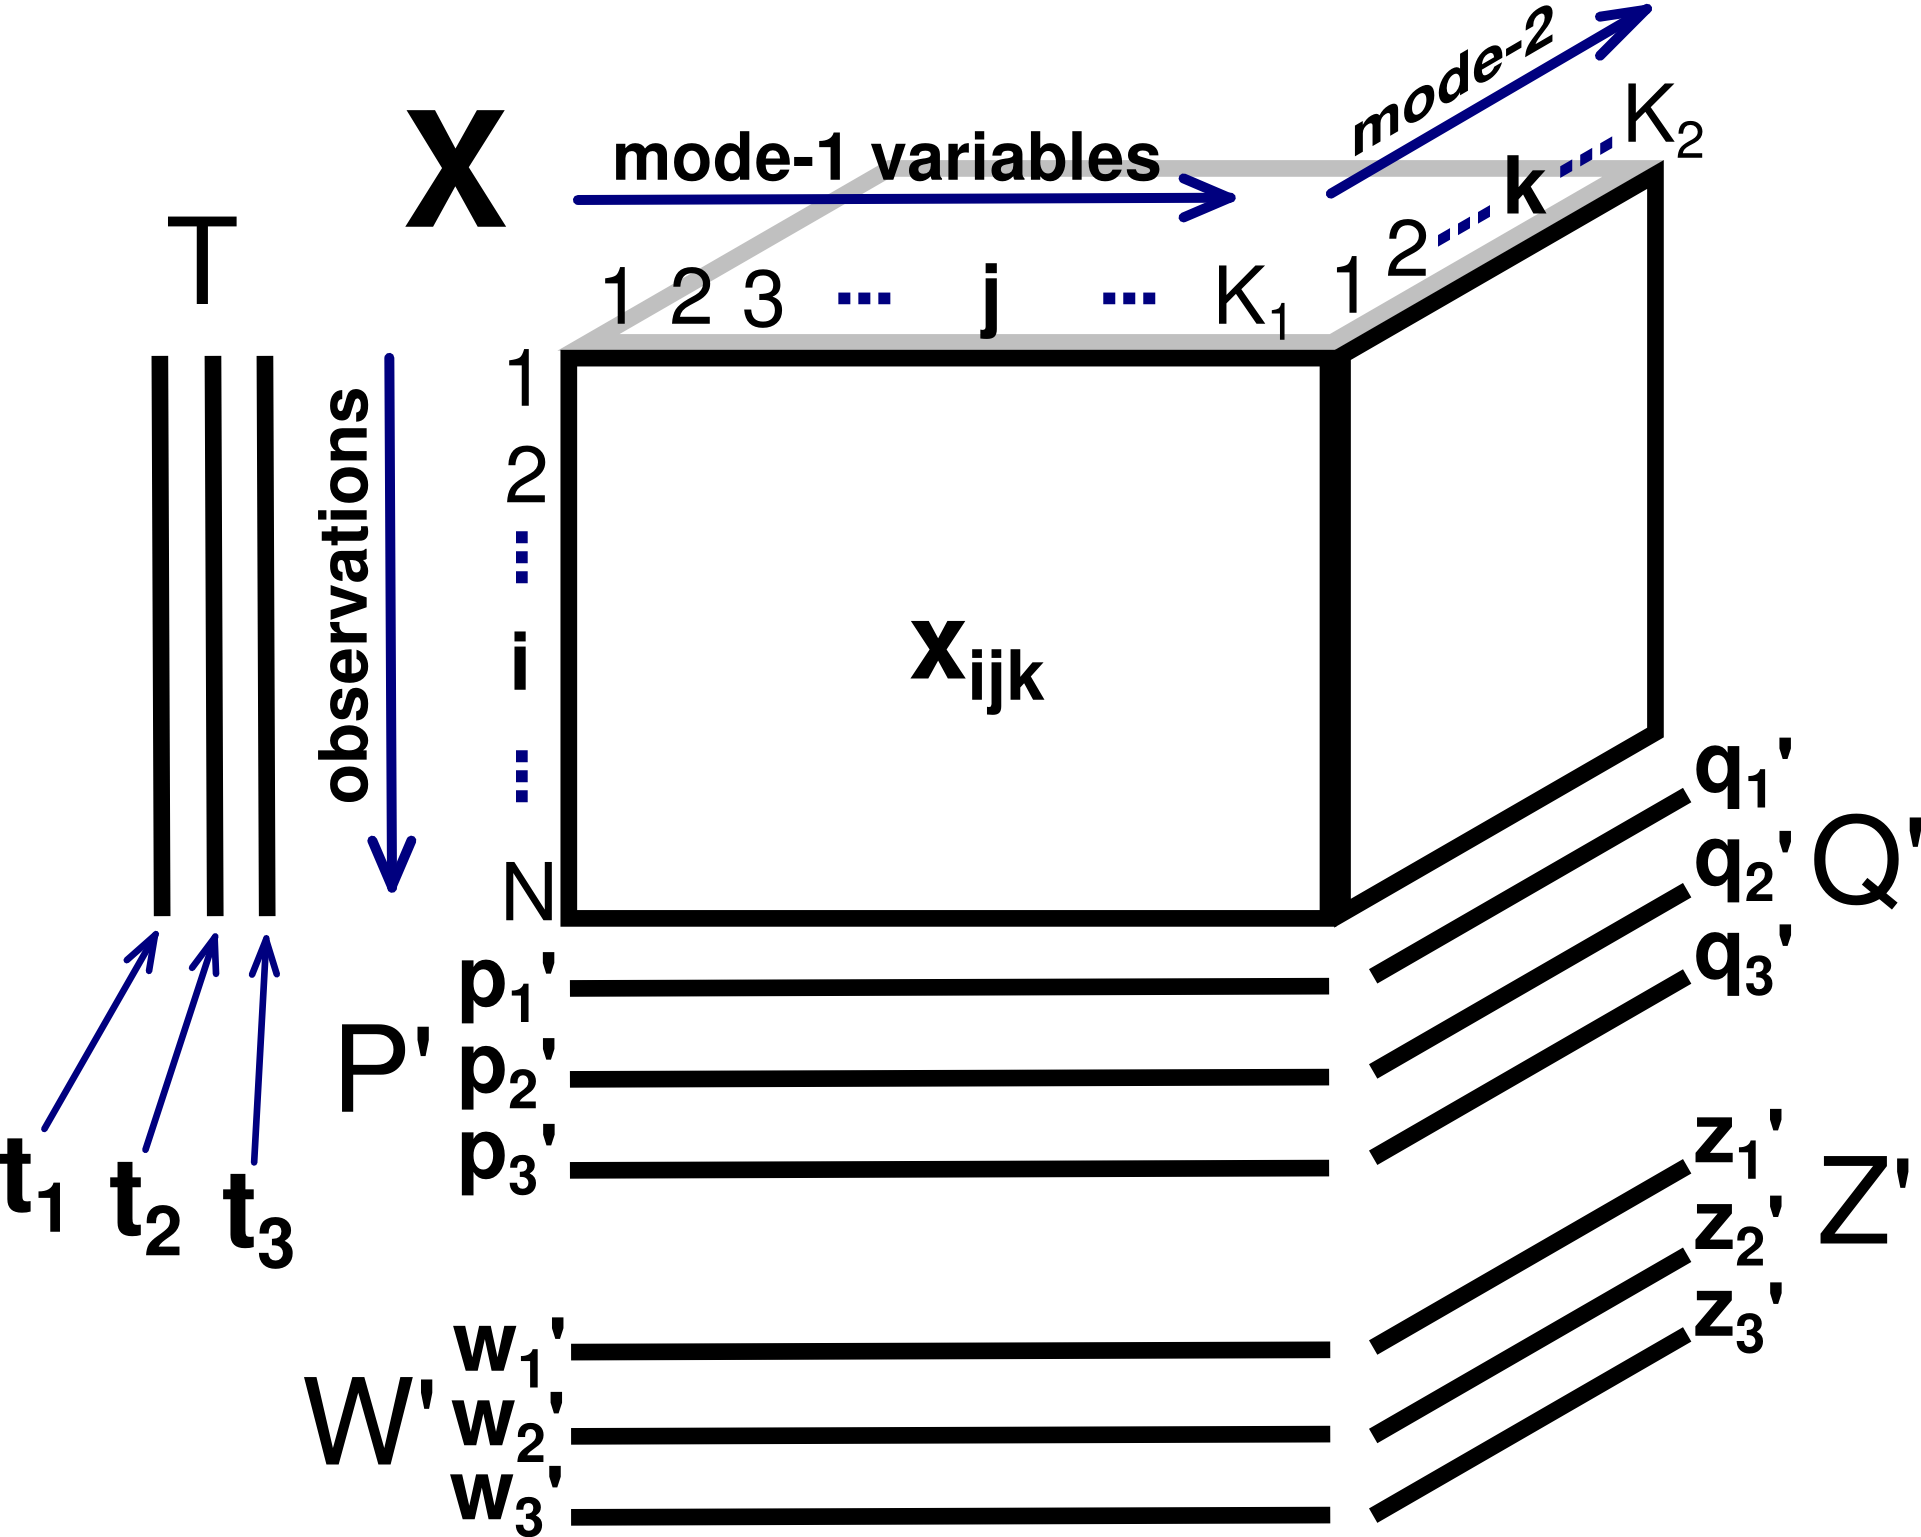
\includegraphics[width=3.5in]{figs/mva/02.png}
\caption
      [Canonical Example of an Unsupervised Trilinear Modeling Problem.]{
  {\bf Canonical Example of an Unsupervised Trilinear Modeling Problem.}
  \\
  Illustration of a third-order data tensor $\mathbf{X}$ as may be found in
  multilinear factorization problems. Such data tensors will contain a set
  of $N$ spectra, each having $K_1$ variables along their first mode and
  $K_2$ variables along their second. The data tensor is then decomposed
  into a small number of score vectors ($\mathbf{t}$) and loading vectors
  ($\mathbf{p}$, $\mathbf{q}$), with corresponding weight vectors
  ($\mathbf{w}$, $\mathbf{z}$) used to transform the observations in
  $\mathbf{X}$ into scores-space. Tick marks denote transposition.
}
\end{SCfigure}

\begin{figure}[hb!]
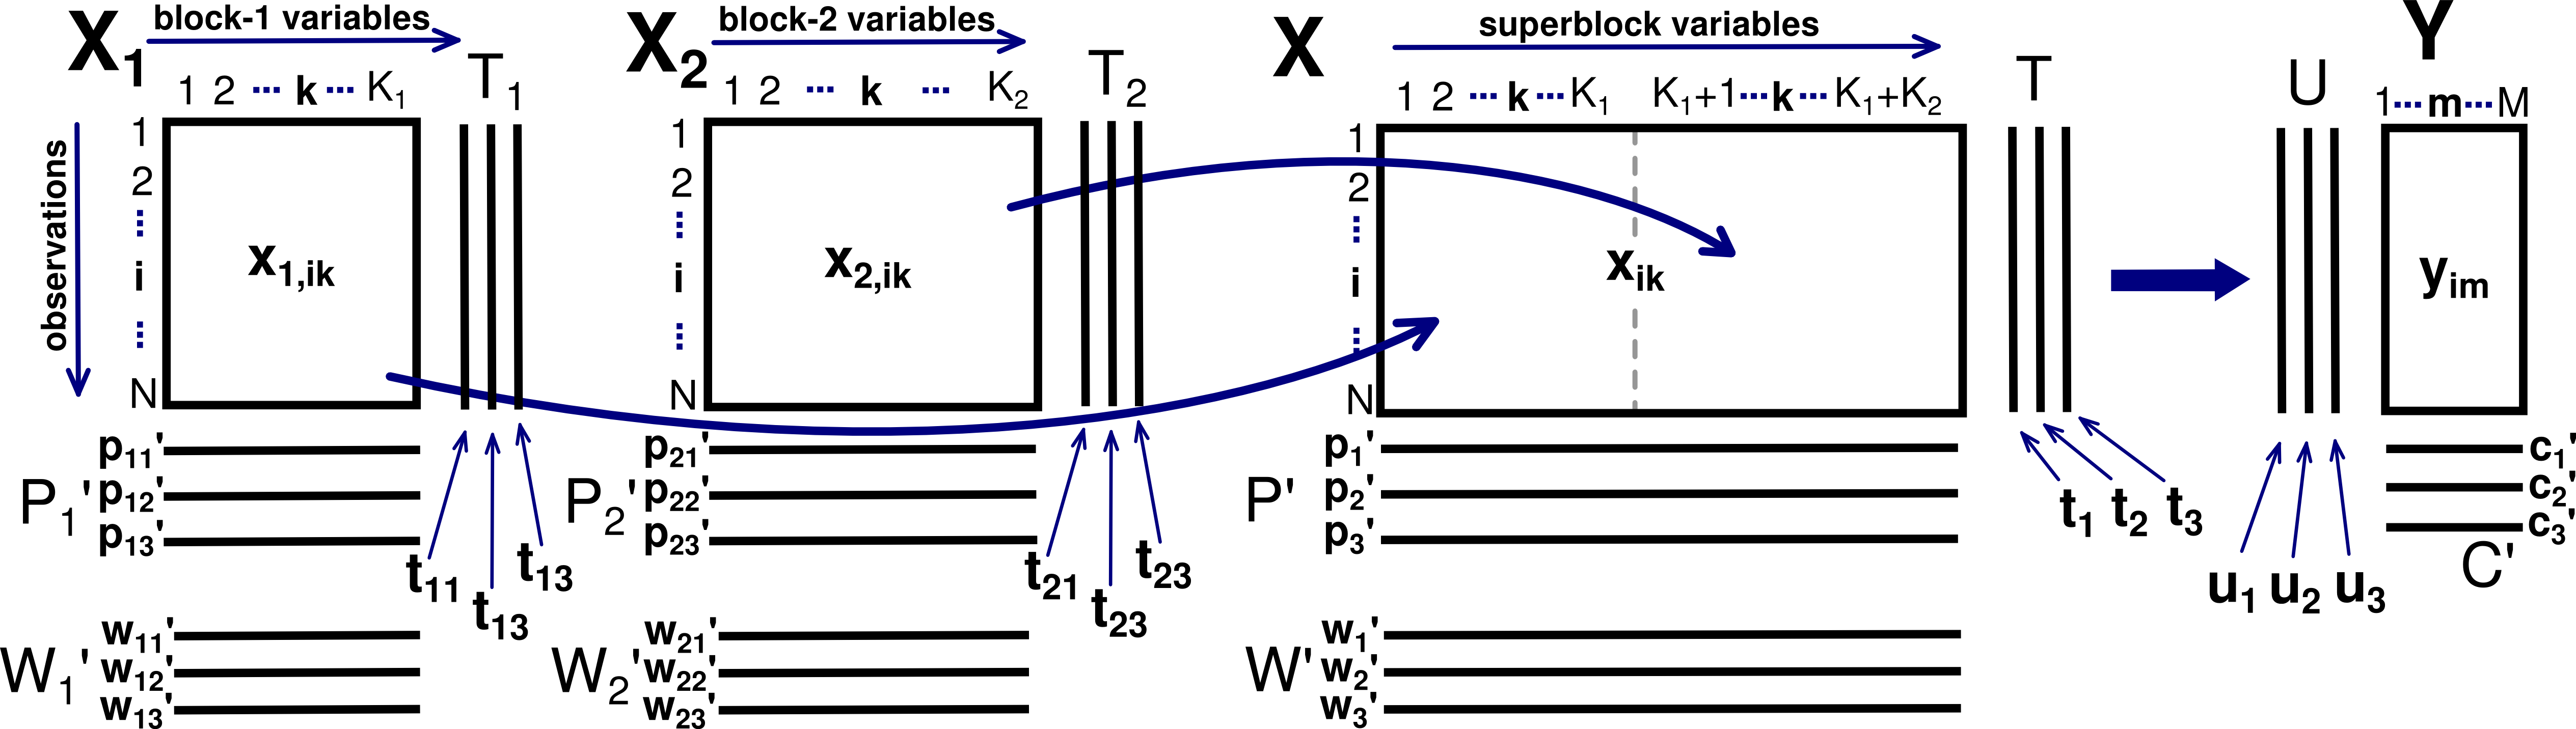
\includegraphics[width=6.5in]{figs/mva/03.png}
\caption
      [Canonical Example of a Multiblock Bilinear Modeling Problem.]{
  {\bf Canonical Example of a Multiblock Bilinear Modeling Problem.}
  \\
  Illustration of a pair of data matrices $\mathbf{X_1}$ and $\mathbf{X_2}$,
  their observation-wise concatenation $\mathbf{X}$, and a response matrix
  $\mathbf{Y}$, as they are typically used in multiblock partial least squares
  modeling problems. In metabolomics applications, each data matrix
  $\mathbf{X_b}$ in the set of $B$ matrices will contain a set of $N$ spectra,
  each having $K_b$ variables. The data are then decomposed into a small number
  of superblock score vectors ($\mathbf{t}$) and superblock loading vectors
  ($\mathbf{p}$), with corresponding superblock weight vectors ($\mathbf{w}$).
  Each individual data matrix is also decomposed into a set of block scores
  ($\mathbf{t_b}$), block loadings ($\mathbf{p_b}$) and block weights
  ($\mathbf{w_b}$). Tick marks denote transposition.
}
\end{figure}

\begin{doublespace}
Another mechanism of increasing the information content of datasets entering
into multivariate chemometric models is to collect spectral observations on
two or more complementary instrumental platforms for each sample. In such a
``multiblock'' modeling approach, each data block $\mathbf{X_b}$ contains $N$
$K_b$-variate observations \cite{westerhuis:jchemo1998,smilde:jchemo2003}.
Bilinear methods such as consensus PCA (CPCA), hierarchical PCA and PLS, and
multiblock PLS may then be used to provide information about data variation
that is correlated between data blocks. Recent examples of multiblock modeling
in metabolomics include fusions of near-IR and mid-IR spectra
\cite{bras:cils2005}, \hnmr{} NMR and direct injection electrospray mass
spectra (DI-ESI-MS, \cite{marshall:metab2015}), and observations from multiple
sensors in process control applications \cite{ferreira:jchemo2010}.
\end{doublespace}

\section{Spectral Processing}

\begin{doublespace}
Following the acquisition of experimental data, instrumentation-specific
processing must be applied to transform the data into a suitable set of
real matrices for bilinear modeling, or tensors for multilinear modeling.
Because the majority of data presented herein originated from an NMR
spectrometer, and because NMR spectra present unique challenges to the
analyst during data handling, the following discussions will center around
processing of 1D and 2D NMR datasets.
\end{doublespace}

\subsection{NMR Signals}

\begin{doublespace}
Modern NMR spectrometers effectively acquire a rotating-frame free induction
decay (FID) through the use of quadrature phase detection of the incoming
signal \cite{levitt2008}. This detection method imparts relative phase
information to the time-domain decays by creating an ``in-phase'' signal
component $i(t)$ and a ``quadrature'' component $q(t)$ phased ninety degrees
from $i(t)$. Indirect dimensions of multidimensional NMR experiments are also
collected in quadrature through interleaved acquisition of one-dimensional
decays that have been cosine- and sine-modulated by the indirect-dimension
signals \cite{states:jmr1982}. As a result, each data point in a
$D$-dimensional NMR signal collected in complete quadrature exists in a
hypercomplex space $\mathbb{H}_D$ \cite{schuyler:jmr2013}, which is defined by
a real basis element and $D$ complex basis elements:

\begin{equation}
\Phi_D \equiv \{ 1 \cdot u_1 \cdots u_D \}
\end{equation}

where multiplication by any complex element $u_d$ results in a ninety degree
phase shift in dimension $d$, and the basis elements combine commutatively
under multiplication, as follows:
\begin{align}
u_i u_j =& u_j u_i \\
u_i^2 =& -1
\end{align}

The basis elements in $\Phi_D$ are a generating set for the complete set of
components of the hypercomplex space $\mathbb{H}_D$. For example, in three
dimensions:

\begin{equation}
\Phi_3 = \{ 1, u_1, u_2, u_1 u_2, u_3, u_1 u_3, u_2 u_3, u_1 u_2 u_3 \}
\end{equation}

A scalar in $\mathbb{H}_D$ is then expressed as a linear combination of this
component set. For the three-dimensional example:

\begin{equation}
x = a + b u_1 + c u_2 + d u_1 u_2
  + e u_3 + f u_1 u_3 + g u_2 u_3 + h u_1 u_2 u_3
\end{equation}

or, more generally and succinctly:

\begin{equation}
x = \sum_{\phi \in \Phi_D} x \{ \phi \} \cdot \phi
\end{equation}

where $x\{\phi\}$ denotes the real coefficient of $x$ that scales the basis
component $\phi$ in $x$. For the above three-dimensional example, the
expression $x\{u_1 u_3\}$ would evaluate to $f$. Finally, the expression of
hypercomplex tensors is formally accomplished by defining each coefficient
as a real tensor of appropriate size, like so:

\begin{equation}
x \{ \phi \} \in \mathbb{R}^{k_1 \cdots k_K} \quad \forall \phi \in \Phi_D
\end{equation}

where $K$ is the number of modes of the tensor. The above equation may be
compactly written as $\mathbb{H}_D^{k_1 \cdots k_K}$. Any scalar
in $\mathbb{H}_D$ -- and therefore any data point in a $D$-dimensional
quadrature-complete NMR dataset -- shall require $2^D$ real coefficients
in order to be completely determined. While the hypercomplex
algebras $\mathbb{H}_0$ and $\mathbb{H}_1$ are isomorphic to the real 
($\mathbb{R}$) and complex ($\mathbb{C}$) numbers, respectively, $\mathbb{H}_2$
and $\mathbb{H}_3$ are {\it not} isomorphic to the quaternions and octonions,
as the latter are noncommutative under multiplication. This hypercomplex
algebra, introduced for partial-component nonuniform subsampling by Schuyler
et al. \cite{schuyler:jmr2013}, provides an elegant formalism for expressing
and handling NMR data.
\\\\
Mathematically, 1D NMR free induction decays are described by the following
commonly used parametric signal model:

\begin{equation}
f(t) = \sum_{m=1}^M \alpha_m \exp\left\{
  u_1 (\omega_m t + \theta_m) - \rho_m t
  \right\}
\end{equation}

where $\alpha_m$, $\omega_m$, $\theta_m$ and $\rho_m$ represent the amplitude,
frequency, phase error and decay rate of the $m$-th damped complex exponential
in the model $f(t)$. Using the above formalism for hypercomplex tensors, this
signal model is trivially extended to any number of dimensions. For example,
a 2D FID may be modeled as follows:

\begin{equation}
f(t_1, t_2) = \sum_{m=1}^M \alpha_m \exp\left\{
  u_1 (\omega_{m,1} t_1 + \theta_{m,1}) +
  u_2 (\omega_{m,1} t_2 + \theta_{m,2}) -
  \rho_{m,1} t_1 - \rho_{m,2} t_2
  \right\}
\end{equation}

In short, NMR free induction decays may be treated as sums of damped
hypercomplex exponentials. While it is possible to directly parameterize
$f(t)$ or $f(t_1, t_2)$ using either maximum likelihood estimation
\cite{chylla:jbnmr1995,chylla:jbnmr1998,chylla:anchem2011} or Bayesian
model selection and estimation
\cite{bretthorst:jmr1990a,
      bretthorst:jmr1990b,
      bretthorst:jmr1990c,
      chylla:jbnmr1993}, this chapter will focus on the soft modeling of
multiple NMR free induction decays using bilinear matrix factorizations.
However, such a description of NMR data is useful in understanding various
processing tasks required by these hypercomplex tensors.
\end{doublespace}

\subsection{Time-domain Processing}

\begin{doublespace}
FIXME. Apodization and first-point scaling, digital filtering, zero-filling.
\end{doublespace}

\subsection{Frequency-domain Processing}

\begin{doublespace}
FIXME. DFT, MEM, phasing, referencing.
\end{doublespace}

\section{Statistical Treatment}

\begin{doublespace}
The properties of the bilinear factorizations commonly applied in metabolomics
dictate that processed data tensors be treated by one or more operations before
they are suitable for modeling. These statistical treatments generally aim to
either reduce the dimensionality of the data tensor (i.e. binning and variable
selection) or increase the self-consistency of observations and variables
(i.e. alignment, normalization and scaling). Treatment operations are usually
instrumentation-agnostic, as the data at this stage of handling almost always
fall into one of the general structures outlined in
\hyperlink{section.3.2}{Section 3.2}.
\end{doublespace}

\subsection{Binning}

\begin{doublespace}
FIXME. Uniform, Optimized, and Intelligent.
\end{doublespace}

\subsection{Alignment}

\begin{doublespace}
FIXME. Warping, global shifting, local shifting. Region selection.
\end{doublespace}

\subsection{Normalization}

\begin{doublespace}
FIXME. CS, PQ, HM, SNV, MSC, (cf. PSC).
\end{doublespace}

\subsection{Scaling}

\begin{doublespace}
FIXME. Centering, UV, Pareto, Range, Level, VAST, MALS.
\end{doublespace}

\subsection{Variable Selection}

\begin{doublespace}
FIXME. Domain knowledge. SVM, GA, RF.
\end{doublespace}

\section{Modeling}

\begin{doublespace}
The most widely applied modeling methods in metabolomics -- namely principal
component analysis, partial least squares and orthogonal projections to latent
structures (OPLS, \cite{trygg:jchemo2002}) -- fall within a class of methods
known as bilinear matrix factorizations. The general form of a bilinear matrix
factorization is:

\begin{equation}
\mathbf{X} = \mathbf{T} \mathbf{P}^T + \mathbf{E}
\end{equation}

where the data matrix $\mathbf{X} \in \mathbb{R}^{N \times K}$ is approximated
by the product of two matrices, $\mathbf{T} \in \mathbb{R}^{N \times A}$ and
$\mathbf{P} \in \mathbb{R}^{K \times A}$, which are referred to as ``scores''
and ``loadings'', respectively. The matrix
$\mathbf{E} \in \mathbb{R}^{N \times K}$ holds any variation in $\mathbf{X}$
that is not captured by the scores and loadings. To understand how such a
factorization may be used to approximate a data matrix, it is instructive to
consider the product of scores and loadings in vector form:

\begin{equation}
\mathbf{X} = \sum_{a=1}^A \mathbf{t_a} \mathbf{p_a}^T + \mathbf{E}
\end{equation}

where $\mathbf{t_a}$ and $\mathbf{p_a}$ are the $a$-th columns of the score
and loading matrices, respectively. In other words, the data matrix is
approximated by a set of $A$ rank-1 matrices that are constructed by the
outer products of each pair of scores and loadings. Because $A$ is commonly
much less than either $N$ or $K$, these bilinear factorizations are also
referred to as low-rank approximations of their data matrices.
\\\\
It is important to note that nearly every data matrix modeled by equation (3.x)
in metabolomics contains far fewer observations than variables
(i.e. $N \ll K$) \cite{worley:cmb2013}. In this situation, there are infinitely
many solutions to the equation that yield the same error $\mathbf{E}$. This is
easily demonstrated by multiplying the scores and loadings by an orthonormal
matrix $\mathbf{R} \in \mathbb{R}^{A \times A}$:

\begin{align}
\mathbf{X}
 =& \: \hat{\mathbf{T}} \hat{\mathbf{P}}^T + \mathbf{E}
\nonumber \\
 =& \: \mathbf{T} \mathbf{R} \mathbf{R}^T \mathbf{P}^T + \mathbf{E}
\nonumber \\
 =& \: \mathbf{T} \mathbf{P}^T + \mathbf{E}
\end{align}

where $\hat{\mathbf{T}} = \mathbf{T} \mathbf{R}$ and
$\hat{\mathbf{P}} = \mathbf{P} \mathbf{R}$. A similar expansion of the solution
set may be accomplished by multiplying the scores by a diagonal $A \times A$
matrix, and multiplying the loadings by the inverse of the same diagonal
matrix. This equivalence of an infinite number of solutions to equation (3.x),
known as the problems of rotational and scale ambiguity, is solved by placing
constraints on the values that scores and loadings may take
\cite{dejuan:aca1997,jolliffe2002}. The choice of constraints defines a
particular bilinear factorization method as unique, and determines what
kind of information is sought from a data matrix using that method.
\end{doublespace}

\subsection{Principal Component Analysis}

\begin{doublespace}
FIXME.
\end{doublespace}

\subsection{Principal Component Regression}

\begin{doublespace}
FIXME.
\end{doublespace}

\subsection{Partial Least Squares}

\begin{doublespace}
FIXME.
\end{doublespace}

\subsection{Orthogonal Projections to Latent Structures}

\begin{doublespace}
FIXME.
\end{doublespace}

\subsection{Multiblock PCA and PLS}

\begin{doublespace}
FIXME.
\end{doublespace}

\section{\hnmr{} NMR Fingerprinting of Brewed Coffees}

\begin{doublespace}
FIXME.
\end{doublespace}

\subsection{Materials and Methods}

\begin{doublespace}
FIXME.
\end{doublespace}

\subsection{Results and Discussion}

\begin{doublespace}
FIXME.
\end{doublespace}

\section{Profiling of Joint \hnmr{} NMR and DI-ESI-MS Data}

\begin{doublespace}
FIXME.
\end{doublespace}

\subsection{Materials and Methods}

\begin{doublespace}
FIXME.
\end{doublespace}

\subsection{Results and Discussion}

\begin{doublespace}
FIXME.
\end{doublespace}

\section{Monte Carlo Analysis of Scores-space Separations}

\begin{doublespace}
FIXME.
\end{doublespace}

\subsection{Materials and Methods}

\begin{doublespace}
FIXME.
\end{doublespace}

\subsection{Results and Discussion}

\begin{doublespace}
FIXME.
\end{doublespace}

\section{Conclusions}

\begin{doublespace}
FIXME.
\end{doublespace}

\bibliographystyle{abbrv}
\bibliography{bworley}

